% ju 28-Mai-22
\documentclass[a4paper,12pt,fleqn,parskip=half]{scrartcl}
\usepackage[ngerman]{babel}
\usepackage[utf8]{inputenc}
\usepackage[T1]{fontenc}

% Schrift
%\usepackage{lmodern}
\usepackage[osf,sc]{mathpazo} 
\usepackage[scale=.9,semibold]{sourcecodepro}   
\usepackage[osf]{sourcesanspro}  

\usepackage[headsepline]{scrlayer-scrpage}
\pagestyle{scrheadings}
\clearpairofpagestyles

\usepackage[table,dvipsnames,usenames]{xcolor}
\usepackage{textcase}
\usepackage{nameref}
\usepackage{hyperref}
\usepackage{tabularx}
\usepackage{multirow}
\usepackage{multicol}
\usepackage{caption, booktabs}
\usepackage{graphicx} 
\usepackage{scrhack}    
\usepackage{url}%% Links
\usepackage[inline]{enumitem}
\usepackage{pifont}
\usepackage{eurosym}% \euro 20,-
\usepackage{amsmath}
\usepackage{amsfonts}
\usepackage{amssymb}
\usepackage{array}            % Extending the array and tabular environments
\usepackage{chngcntr}         % Change the resetting of counters
\usepackage[version=4]{mhchem}
\usepackage{stmaryrd}
\usepackage{siunitx}
\usepackage{float}
\usepackage{csquotes}
\usepackage{subcaption}
\usepackage{mathtools}
\usepackage{icomma}%Dezimaltrennzeichen
\usepackage{multimedia}%Video: \movie[externalviewer]{(video.mov)}{video.mov}
\usepackage{epstopdf}
\usepackage{footnote}
\usepackage{qrcode}% Anwendung: \qrcode[hyperlink,level=Q,version=2,height=1cm]{\website}
\usepackage{underscore}% Unterstrich ____

% PDF Dokumente einbinden
\usepackage{pdfpages}% \includepdf[pages=-]{Tabellen/Excel.pdf}
\RequirePackage{lastpage}  % Pagecounter

\addto\captionsngerman{%
\renewcommand{\figurename}{Abb.}
\renewcommand{\tablename}{Tab.}
}

% listings
\usepackage{listings}
\lstset{basicstyle=\linespread{1}\ttfamily\small,floatplacement=!htb,captionpos=t,abovecaptionskip=.5\baselineskip,belowcaptionskip=.5\baselineskip,upquote=true,showstringspaces=false,inputencoding=utf8,tabsize=4,
    	keywordstyle=\bfseries ,
	commentstyle=\color{rot5},
	stringstyle=\color{orange},
	breaklines=true,
  	postbreak=\mbox{\textcolor{black}{$\hookrightarrow$}\space},
	breakatwhitespace=false
}
\lstset{literate={á}{{\'a}}1 {é}{{\'e}}1 {í}{{\'i}}1 {ó}{{\'o}}1 {ú}{{\'u}}1 {Á}{{\'A}}1 {É}{{\'E}}1 {Í}{{\'I}}1 {Ó}{{\'O}}1 {Ú}{{\'U}}1 {à}{{\`a}}1 {è}{{\`e}}1 {ì}{{\`i}}1 {ò}{{\`o}}1 {ù}{{\`u}}1 {À}{{\`A}}1 {È}{{\'E}}1 {Ì}{{\`I}}1 {Ò}{{\`O}}1 {Ù}{{\`U}}1 {ä}{{\"a}}1 {ë}{{\"e}}1 {ï}{{\"i}}1 {ö}{{\"o}}1 {ü}{{\"u}}1 {Ä}{{\"A}}1 {Ë}{{\"E}}1 {Ï}{{\"I}}1 {Ö}{{\"O}}1 {Ü}{{\"U}}1 {â}{{\^a}}1 {ê}{{\^e}}1 {î}{{\^i}}1 {ô}{{\^o}}1 {û}{{\^u}}1 {Â}{{\^A}}1 {Ê}{{\^E}}1 {Î}{{\^I}}1 {Ô}{{\^O}}1 {Û}{{\^U}}1 {œ}{{\oe}}1 {Œ}{{\OE}}1 {æ}{{\ae}}1 {Æ}{{\AE}}1 {ß}{{\ss}}1 {ű}{{\H{u}}}1 {Ű}{{\H{U}}}1 {ő}{{\H{o}}}1 {Ő}{{\H{O}}}1 {ç}{{\c c}}1 {Ç}{{\c C}}1 {ø}{{\o}}1 {å}{{\r a}}1 {Å}{{\r A}}1 {€}{{\EUR}}1 {£}{{\pounds}}1 {~}{{\textasciitilde}}1 {-}{{-}}1 }

% bibliography
\usepackage[
    bibencoding=utf8,
    backend=biber,% bibtex, biber
    backref=false,backrefstyle=three+,url=true,urldate=comp,abbreviate=false,maxnames=20
]{biblatex} %Paket laden
\DeclareBibliographyCategory{cited}
\let\defaultcite\cite\renewcommand*\cite[2][]{\addtocategory{cited}{#2}\defaultcite[#1]{#2}}
\let\defaulttextcite\textcite\renewcommand*\textcite[2][]{\addtocategory{cited}{#2}\defaulttextcite[#1]{#2}}
\setcounter{biburllcpenalty}{7000}
\setcounter{biburlucpenalty}{8000}
\AfterPackage{biblatex}{
	\PreventPackageFromLoading[\errmessage{Sie haben versucht, das Cite-Paket zu laden, das nicht mit biblatex kompatibel ist.}]{cite}
}

\hypersetup{%
	%pdftitle={\titel},
	%pdfsubject={Latex},
	%pdfauthor={\autor},
	%pdfcreator={\autor}, 
	bookmarksnumbered=true,
	breaklinks=true,
	%colorlinks=true,	   
	linkcolor=rot5,		
	filecolor=blau5,		
	urlcolor=blau5,			
	citecolor=ForestGreen
}

\linespread{1.1}
\setlist{itemsep=0pt}
\widowpenalty10000
\clubpenalty10000
\tolerance1000   

\usepackage[left=2cm,right=2cm,top=1cm,bottom=1cm,includeheadfoot]{geometry}
%\usepackage[left=4cm,right=2cm,top=1cm, bottom=1cm,includeheadfoot]{geometry}
%\usepackage[left=6cm,right=1cm,top=1cm, bottom=1cm,includeheadfoot]{geometry}
%\usepackage[landscape=true,left=2cm,right=2cm,top=1cm,bottom=1cm,includeheadfoot]{geometry}%quer

% eigene Farbe definieren
% Adobe Prozessfarben: CMYK: 100,50,0,35 -> 1,0.5,0,0.35
\definecolor{orange}{cmyk}{0,0.55,0.61,0}   % 0,55,61,0
\definecolor{blau5}{cmyk}{1,0.77,0.1,0.01}  % 100,77,10,
\definecolor{rot5}{cmyk}{0.22,1,1,0.19}     % 22,100,100,19
\definecolor{grau2}{cmyk}{0,0,0,0.1}        % 0,0,0,40
\definecolor{blau}{cmyk}{0.93,0.66,0,0.21}% 

% Literatur
\bibliography{content/literatur}
\bibliography{content/literatur-kfz}
\bibliography{content/literatur-sport}

%%%%%%%%%%%%%%%%%%%%%%%%%%%%%%%%%%%%%%%%%%%%%%%%%%%%%%%
\newcommand{\name}{Jan Unger}% anpassen!!!!!
\newcommand{\thema}{01-Grundlagen-Elektrik}
\newcommand{\quelle}{\name}
\newcommand{\website}{https://bw-ju.de/}
\newcommand{\github}{https://github.com/ju1-eu}
%%%%%%%%%%%%%%%%%%%%%%%%%%%%%%%%%%%%%%%%%%%%%%%%%%%%%%%

\ihead{\textbf{Quelle:} \quelle}%{Kopfzeile innen}
\ohead{\textbf{Datum:} \today}  %{Kopfzeile außen}

\ifoot{\textbf{Thema:} \thema}  %{Fußzeile  innen}
\ofoot{Seite {\thepage} von {\pageref{LastPage}}}%{Fußzeile  außen}

\title{\thema}
\author{\name}
\date{\today}

\begin{document}
	%\thispagestyle{empty}
	%\maketitle
	%\newpage
	%\setcounter{page}{1}

	%%%%%%%%%%%%%%%%%%%%%%%%%%%%%%%%%%%%%%%%%%%
	\begin{center}
		\textbf{\Large \thema}%14pt
		\vspace{0.8em}
		
		%\datum	
		%\qrcode[hyperlink,level=Q,version=2,height=1cm]{\website}
		\qrcode[hyperlink,level=Q,version=2,height=1cm]{\github}
	\end{center}
	%%%%%%%%%%%%%%%%%%%%%%%%%%%%%%%%%%%%%%%%%%%

	\subsection*{Keywords}%\label{sec:Deadline}\index{Deadline}
	% Checkliste
	\begin{itemize}[label=\checkmark] %\itemsep -2pt
		\item Begriff 
	\end{itemize}

    %%%%%%%%%%%%%%%%%%%%%%%%%%%%%%%%%%%%%%%%%%%%%%%%%%%%%%%%%%%%%%%%%%

	% anpassen
	%\input{content/tex/neu}
	%ju 28-Mai-22 01-Grundlagen-Elektrik.tex
\section{Die elektrische Spannung}\label{die-elektrische-spannung}

\textbf{Spannung} $U \quad \text{[Volt]} \quad [V]$

\emph{italienischer Physiker Alessandro Volta (1745-1827)}

\begin{table}[!ht]% hier: !ht 
\centering 
	\caption{}% \label{tab:}%% anpassen 
\begin{tabular}{@{}llll@{}}
\hline
\textbf{Einheit} & \textbf{Abk.} & \textbf{Zahl} &
\textbf{Exponentialschreibweise} \\
\hline
kilo V & $[KV]$ & $1000~V$ & $\num{1,0e3}~V$ \\
Volt & $[V]$ & $1~V$ & $\num{1,0e0}~V$ \\
milli V & $[mV]$ & $0,001~V$ & $\num{1,0e-3}~V$ \\
\hline
\end{tabular} 
\end{table}

In einer Spannungsquelle, z.~B. Drehstromgenerator, werden die
unterschiedlichen Ladungen unter Energieaufwand (Drehbewegung,
Magnetismus) voneinander getrennt.

Es bilden sich zwei Pole aus.

\begin{itemize}
\item
  Negativer Pol: hier herrscht Elektronenüberschuss
\item
  Positiver Pol: Elektronenmangel
\end{itemize}

Man spricht hierbei auch von dem Vorhandensein einer Potentialdifferenz.

Diese beiden Ladungen haben das Bestreben sich auszugleichen, dieses
Ausgleichsbestreben bezeichnet man als elektrische Spannung.

\textbf{Messen}

Das Spannungsmessgerät wird grundsätzlich parallel zum Messobjekt
geschaltet.

\emph{Besonderheit}: Spannungsmessgeräte besitzen ein sehr hochohmigen
Innenwiderstand (Impedanz).

\newpage

\section{Der elektrische Strom}\label{der-elektrische-strom}

\textbf{Strom} $I \quad \text{[Ampere]} \quad [A]$

\emph{französischer Physiker André-Marie Ampère (1775-1836)}

I = Intensität, International >>Ampere<<

\begin{table}[!ht]% hier: !ht 
\centering 
	\caption{}% \label{tab:}%% anpassen 
\begin{tabular}{@{}llll@{}}
\hline
\textbf{Einheit} & \textbf{Abk.} & \textbf{Zahl} &
\textbf{Exponentialschreibweise} \\
\hline
kilo A & $[KA]$ & $1000~A$ & $\num{1,0e3}~A$ \\
Ampere & $[A]$ & $1~A$ & $\num{1,0e0}~A$ \\
milli A & $[mA]$ & $0,001~A$ & $\num{1,0e-3}~A$ \\
micro A & $[\mu A]$ & $0,000001~A$ & $\num{1,0e-6}~A$ \\
nano A & $[nA]$ & $0,000000001~A$ & $\num{1,0e-9}~A$ \\
\hline
\end{tabular} 
\end{table}

Der elektrische Strom ist die gerichtete Bewegung von freien Elektronen.

Ursache des elektrischen Stroms ist die elektrische Spannung.
Elektrischer Strom kann nur im geschlossenen Stromkreis fließen. Ein
Stromkreis besteht mindestens aus dem Spannungserzeuger, dem Verbraucher
und den Leitungen.

Fuse (Sicherung: T = Träge, f = schnell, ff = superschnell)

\textbf{Messen}

Das Strommessgerät wird in Reihe zum Messobjekt geschaltet.

\emph{Besonderheit}:

Strommessgeräte besitzen einen sehr niederohmigen Innenwiderstand.

\newpage

\section{Der elektrische Widerstand}\label{der-elektrische-widerstand}

\textbf{Widerstand} $R \quad \text{[Ohm]} \quad [\Omega]$

\emph{deutsche Physiker Georg Simon Ohm (1789-1854)}

resistor = Widerstand

\begin{table}[!ht]% hier: !ht 
\centering 
	\caption{}% \label{tab:}%% anpassen 
\begin{tabular}{@{}llll@{}}
\hline
\textbf{Einheit} & \textbf{Abk.} & \textbf{Zahl} &
\textbf{Exponentialschreibweise} \\
\hline
Mega $\Omega$ & $[M\Omega]$ & $1000000~\Omega$ &
$\num{1,0e6}~\Omega$ \\
Kilo $\Omega$ & $[K\Omega]$ & $1000~\Omega$ &
$\num{1,0e3}~\Omega$ \\
Ohm & $[\Omega]$ & $1~\Omega$ & $\num{1,0e0}~\Omega$ \\
milli $\Omega$ & $[m\Omega]$ & $0,001~\Omega$ &
$\num{1,0e-3}~\Omega$ \\
\hline
\end{tabular} 
\end{table}

Bewegen sich Elektronen durch einen Leiter, so prallen sie auf ihrem Weg
durch den Leiter ständig mit den Atomen des Leiterwerkstoffes zusammen,
sie werden also auf ihrem Weg durch den Leiter gehemmt. Dieses behindern
der Ladungsträger bezeichnet man als elektrischer Widerstand.

\begin{figure}[!ht]% hier: !ht
\centering
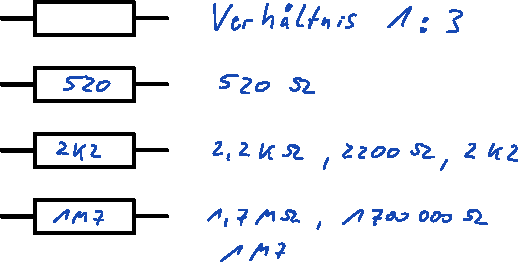
\includegraphics[width=0.3\textwidth]{images/Skizze/15_Schaltzeichen_Widerstand_Skizze.pdf}
\caption{Schaltzeichen Widerstand}
%\label{fig:}%% anpassen
\end{figure}

\begin{figure}[!ht]% hier: !ht
\centering
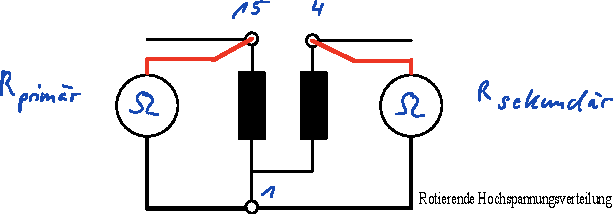
\includegraphics[width=0.6\textwidth]{images/Skizze/16_Widerstandsmessung_Skizze.pdf}
\caption{Widerstandsmessung}
%\label{fig:}%% anpassen
\end{figure}

\textbf{Messen}

Das Widerstandsmessgerät wird parallel zum Messobjekt geschaltet.

\emph{Messvoraussetzung}:

Das Messobjekt muss aus dem Stromkreis heraus gelöst sein und sich im
spannungsfreien Zustand befinden.

\textbf{Einsatzmöglichkeiten von Widerständen}

\emph{Reihe}

\begin{enumerate}
\def\labelenumi{(\arabic{enumi})}
\item
  Strombegrenzung
\item
  Spannungsteilung
\end{enumerate}

\emph{Parallel}

\begin{enumerate}
\def\labelenumi{(\arabic{enumi})}
\item
  Stromflusserhöhung
\item
  Leistungsteilung $\boxed{R_{ges} = \frac{R_{Teil}}{n}}$ (z. B.
  $n = 2 \to$ Leistung halbieren)
\end{enumerate}

\begin{figure}[!ht]% hier: !ht
\centering
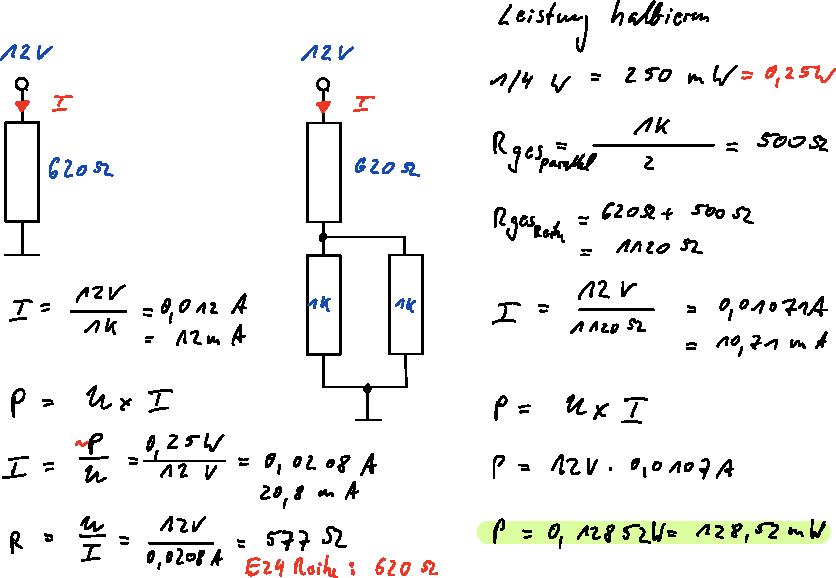
\includegraphics[width=0.6\textwidth]{images/Skizze/17_Leistungsteilung_Skizze.pdf}
\caption{Leistungsteilung}
%\label{fig:}%% anpassen
\end{figure}

\begin{figure}[!ht]% hier: !ht
\centering
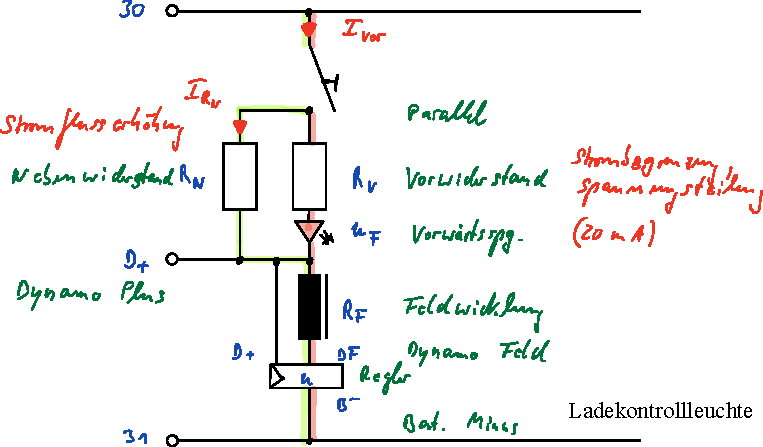
\includegraphics[width=0.6\textwidth]{images/Skizze/18_Stromflusserhoehung_Strombegrenzung_Spannungsteilung_Skizze.pdf}
\caption{Stromflusserhöhung, -begrenzung, Spannungsteilung}
%\label{fig:}%% anpassen
\end{figure}

\newpage

\section{Stromflussrichtungen}\label{stromflussrichtungen}

\begin{figure}[!ht]% hier: !ht
\centering
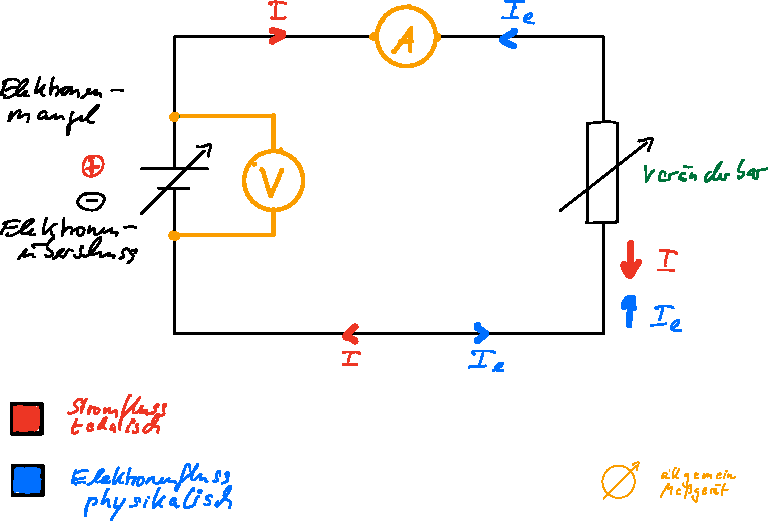
\includegraphics[width=0.6\textwidth]{images/Skizze/06_Stromfluss_Messen_Skizze.pdf}
\caption{Stromfluss und Messen}
%\label{fig:}%% anpassen
\end{figure}

\textbf{Technische Stromflussrichtung} der Strom fließt von plus nach
minus

\textbf{physikalische Stromflussrichtung} tatsächlicher Elektronenfluss,
die Elektronen bewegen sich von minus nach plus

\newpage

\section{Normgerechte Darstellung des Stromflusses durch einen
Leiter}\label{normgerechte-darstellung-des-stromflusses-durch-einen-leiter}

$\otimes$ Strom fließt vom Betrachter weg

$\odot$ Strom fließt auf den Betrachter zu

\section{Magnetfeld eines stromdurchflossenen
Leiters}\label{magnetfeld-eines-stromdurchflossenen-leiters}

Magnetfeldrichtung festlegen

\begin{figure}[!ht]% hier: !ht
\centering
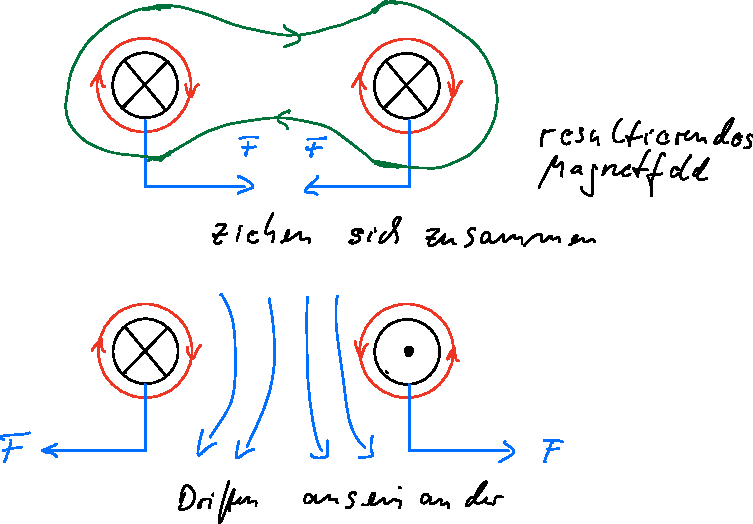
\includegraphics[width=0.6\textwidth]{images/Skizze/05_StromdurchflossenerLeiter_Skizze.pdf}
\caption{Stromdurchflossener Leiter}
%\label{fig:}%% anpassen
\end{figure}

\section{Normgerechte Festlegung des Nordpols einer stromdurchflossenen
Spule}\label{normgerechte-festlegung-des-nordpols-einer-stromdurchflossenen-spule}

\begin{figure}[!ht]% hier: !ht
\centering
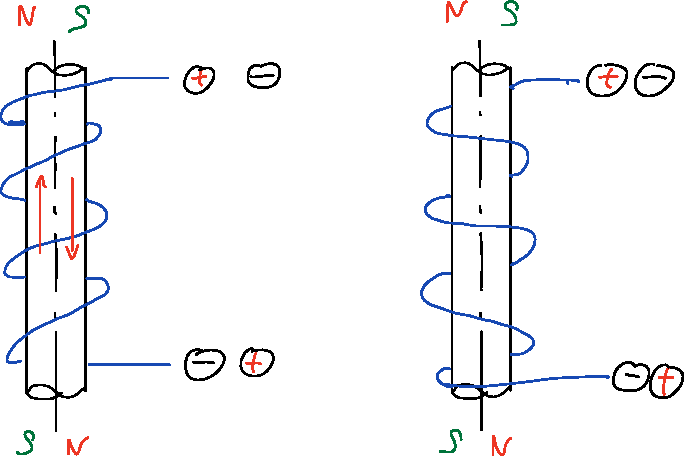
\includegraphics[width=0.6\textwidth]{images/Skizze/03_StromdurchflosseneSpule_Skizze.pdf}
\caption{Stromdurchflossene Spule}
%\label{fig:}%% anpassen
\end{figure}

Umfasst man mit der rechten Hand eine stromdurchflossene Spule so, dass
die Finger in Stromflussrichtung zeigen (technische Stromflussrichtung),
so zeigt der abgespreizte Daumen in Richtung des Nordpols.

\newpage

\section{Rechte Hand-Regel
(Generatorregel)}\label{rechte-hand-regel-generatorregel}

\begin{figure}[!ht]% hier: !ht
\centering
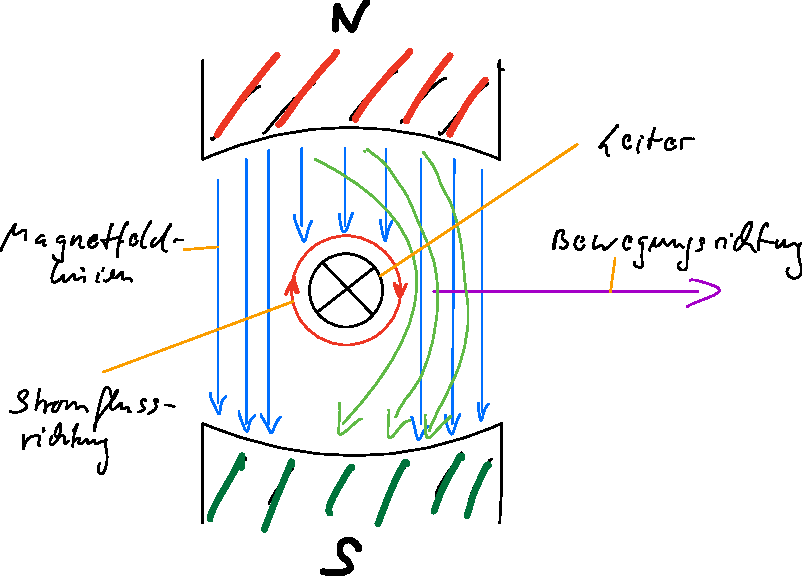
\includegraphics[width=0.6\textwidth]{images/Skizze/01_Generatorregel_Skizze.pdf}
\caption{Generatorregel}
%\label{fig:}%% anpassen
\end{figure}

Hält man die rechte Hand so in ein Magnetfeld, sodass der Nordpol in die
Handinnenfläche eintrifft. Und übt man dabei eine Bewegung in Richtung
des abgespreizten Daumens aus, so fließt ein Strom in Richtung der
Fingerspitzen.

\section{Linke Hand Regel
(Motorregel)}\label{linke-hand-regel-motorregel}

\begin{figure}[!ht]% hier: !ht
\centering
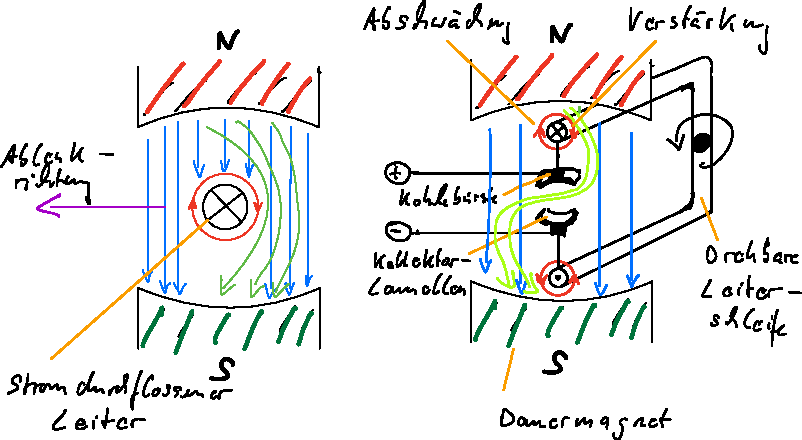
\includegraphics[width=0.6\textwidth]{images/Skizze/02_Motorregel_Skizze.pdf}
\caption{Motorregel}
%\label{fig:}%% anpassen
\end{figure}

Hält man die linke Hand so in ein Magnetfeld, dass der Nordpol in die
Handinnenfläche eintrifft und fließt dabei ein Strom in Richtung der
Fingerspitzen, so wird der Leiter in Richtung des abgespreizten Daumens
aus dem Magnetfeld abgelenkt.

\section{Das ohmsche Gesetz}\label{das-ohmsche-gesetz}

Im ohmschen Widerstand sind die Beziehungen zwischen Strom, Spannung und
Widerstand im Stromkreis festgelegt. Die Stromstärke steigt mit
zunehmender Spannung und sinkt mit zunehmendem Widerstand.

$\boxed{I = \frac{U}{R}} \quad \bigl[\frac{V}{\Omega}\bigl] = A \quad  \boxed{R = \frac{U}{I}} \quad \bigl[\frac{V}{A}\bigl] = \Omega \quad  \boxed{U = R \cdot I} \quad [\Omega \cdot A] = V$

\newpage

\section{Stromdichte J}\label{stromdichte-j}

\begin{figure}[!ht]% hier: !ht
\centering
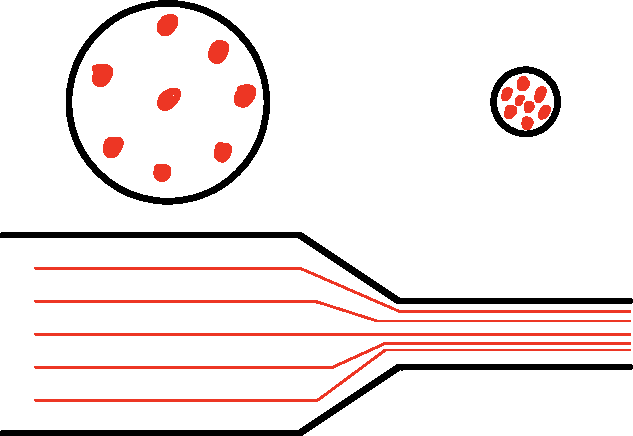
\includegraphics[width=0.4\textwidth]{images/Skizze/04_Stromdichte_Skizze.pdf}
\caption{Stromdichte}
%\label{fig:}%% anpassen
\end{figure}

\begin{itemize}
\item
  \textbf{Große Fläche}

  \begin{itemize}
  \item
    Kleine Stromdichte
  \end{itemize}
\item
  \textbf{Kleine Fläche}

  \begin{itemize}
  \item
    Große Stromdichte
  \end{itemize}
\end{itemize}

Unter Stromdichte versteht man die Anzahl der Ladungsträger Elektronen
pro Flächeninhalt $mm^2$ . Die Stromdichte ist die Ursache der
Erwärmung eines leitenden Stoffes. Ist die zu groß, wird oder kann der
Leiter zerstört werden.

\textbf{Erlaubte Stromdichte Werte:}

$J_{\text{zulässig}} = 10~\frac{A}{mm^2} \,\text{bei Kurzzeitbelastung}$

$J_{\text{zulässig}} = 30~\frac{A}{mm^2} \,\text{zugelassen (Starter)}$

\textbf{Formel}

$\boxed{J = \frac{I}{A}} \quad \bigl[\frac{A}{mm^2}\bigl] \quad  \boxed{I = J \cdot A} \quad \bigl[\frac{A \cdot mm^2}{mm^2} = A\bigl] \quad  \boxed{A = \frac{I}{J}} \quad \bigl[\frac{A \cdot mm^2}{A} = mm^2\bigl]$

\section{Leitwert G}\label{leitwert-g}

Der Leitwert ist das Vermögen eines Widerstandes einen Strom fließen
lassen zu können. Ein >>hochohmiger Widerstand<< lässt einen kleinen
Stromfluss zu. Der besitzt also einen kleinen Leitwert. Und umgekehrt
ein >>niederohmiger Widerstand<<, lässt einen hohen Stromfluss zu. Der
besitzt einen großen Leitwert. Der Leitwert ist der Kehrwert des
Widerstandes.

\textbf{Formel}

$\boxed{G = \frac{1}{R}} \quad \bigl[\frac{1}{\Omega} = S\bigl] \,\text{Siemens} \quad \boxed{R = \frac{1}{G}} \quad \bigl[\frac{1}{S} = \Omega\bigl]$

\section{Leiterwiderstand}\label{leiterwiderstand}

\emph{Abhängig}

\begin{enumerate}
\item
  Leiterlänge $l~[m] \quad R_l \sim l$
\item
  Leiterfläche $A~[mm^2] \quad R_l \sim \frac{1}{A}$
\item
  Werkstoff - spezifische Widerstand
  $\rho~\text{(rho)}~\bigl[\frac{\Omega \cdot mm^2}{m}\bigl] \quad R_l \sim \rho$
\end{enumerate}

\emph{Aluminium} $\rho_{Al} = 0,0278~\frac{\Omega \cdot mm^2}{m}$ ist
hochohmiger als \emph{Kupfer}
$\rho_{cu} = 0,0178~\frac{\Omega \cdot mm^2}{m}$.

\textbf{Leiterwiderstand R}

Er hängt von der Leiterlänge, vom spezifischen Widerstand und dem
Leiterquerschnitt ab.

\textbf{Spezifische Widerstand $\rho$ (rho)}

Ist der Widerstand eines Leiters von $1~m$ Länge und $1~mm^2$
Querschnitt.

\textbf{Formel}

$\boxed{R_l = \frac{\rho \cdot l}{A}} \, \bigl[\frac{\Omega \cdot mm^2 \cdot m}{m \cdot mm^2} = \Omega\bigl] \boxed{A = \frac{\rho \cdot l}{R_l}} \, \bigl[\frac{\Omega \cdot mm^2 \cdot m}{m \cdot \Omega} = mm^2\bigl] \boxed{l = \frac{R_l \cdot A}{\rho}} \, \bigl[\frac{\Omega \cdot mm^2 \cdot m}{\Omega \cdot mm^2} = m\bigl]$

\newpage

\section{Reihenschaltung von
Widerständen}\label{reihenschaltung-von-widerstaenden}

\begin{figure}[!ht]% hier: !ht
\centering
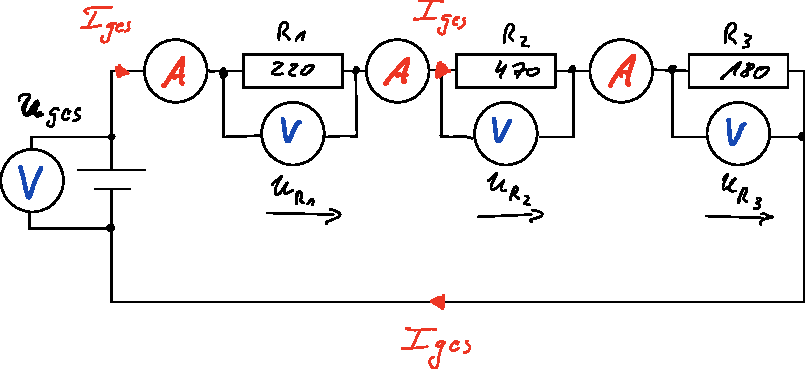
\includegraphics[width=0.6\textwidth]{images/Skizze/07_Reihenschaltung_Widerstaende_Skizze.pdf}
\caption{Reihenschaltung - Widerstände}
%\label{fig:}%% anpassen
\end{figure}

$\boxed{U = R \cdot I}$

Werden mehrere verschieden - große oder gleich große Widerstände in
Reihe geschaltet, so fällt an jedem Widerstand nach Größe des
Widerstands eine Spannung ab, die addiert die Gesamtspannung ergibt.

$\boxed{U_{ges} = U_{R_1} + U_{R_2} + U_{R_3} + \dots + U_{R_n}} \quad \bigl[V + V + V\bigl] = V$

Möchte man den Spannungsabfall an gleich großen in Reihe geschalteten
Widerständen berechnen, kann nachfolgende Gleichung verwendet werden.

$\boxed{U_{teil} = \frac{U_{ges}}{n}} \quad \bigl[\frac{V}{1}\bigl] = V$

Die Stromstärke ist an jedem Punkt des Stromkreises gleich groß, d.h.
durch jeden Widerstand fließt die gleiche Stromstärke.

$\boxed{I_{ges} = I_{R_1} = I_{R_2} = I_{R_3} = \dots = I_{R_n}} \quad \bigl[A = A = A\bigl] = A$

Der Gesamtwiderstand der Schaltung setzt sich aus der Addition der
Teilwiderstände zusammen.

$\boxed{R_{ges} = R_1 + R_2 + R_3 + \dots + R_n} \quad \bigl[\Omega + \Omega + \Omega\bigl] = \Omega$

\textbf{Rechenbeispiel}

geg:

$U_{ges} = 13,8~V$

$R_1 = 220~\Omega, R_2 = 470~\Omega, R_3 = 180~\Omega$

ges: $R_{ges}, I, U_1, U_2, U_3$

Formel

$R_{ges} = R_1 + R_2 + R_3$

$I = \frac{U_{ges}}{R_{ges}}$

$U_1 = R_1 \cdot I, U_2 = R_2 \cdot I, U_3 = R_3 \cdot I$

Lösung:

$R_{ges} = 870~\Omega$

$I = 0,0159~A$

$U_1 = 3,4897~V, U_2 = 7,4552~V, U_3 = 2,8552~V$

\newpage

\section{Relais}\label{relais}

\textbf{Arten}

\begin{enumerate}
\item
  Spannungsrelais (Schließer, Öffner, Wechsler)
\item
  Stromrelais
\end{enumerate}

\textbf{Aufgaben}

\begin{enumerate}
\item
  kleiner Spannungsabfall
\item
  kein Einfluss auf Verbraucher
\end{enumerate}

\subsection{Spannungsrelais}\label{spannungsrelais}

\begin{figure}[!ht]% hier: !ht
\centering
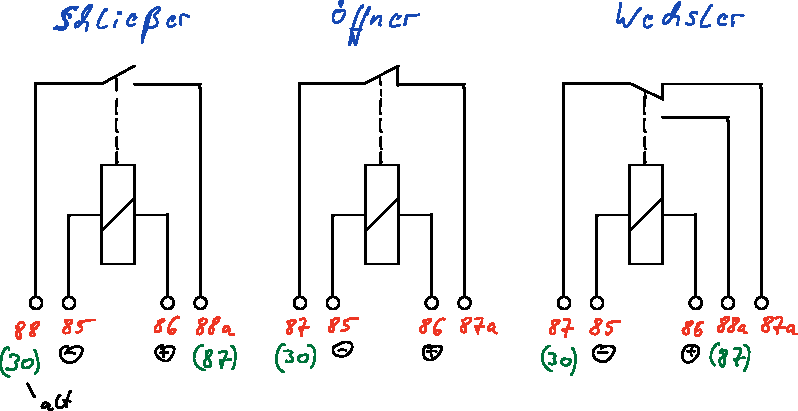
\includegraphics[width=0.7\textwidth]{images/Skizze/08_Relais_Skizze.pdf}
\caption{Relais}
%\label{fig:}%% anpassen
\end{figure}

\textbf{Ströme einer Relaisschaltung}

\begin{figure}[!ht]% hier: !ht
\centering
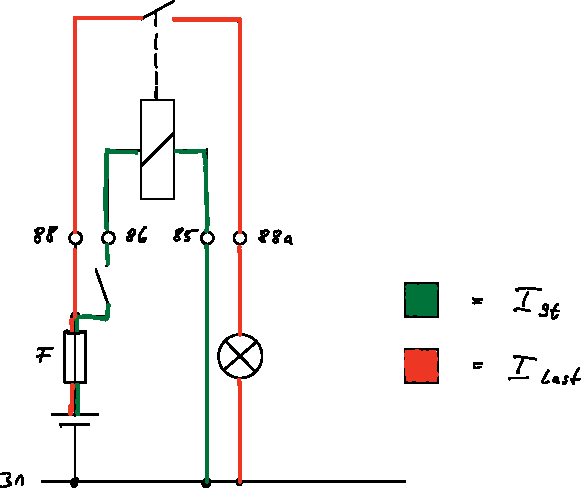
\includegraphics[width=0.4\textwidth]{images/Skizze/09_Stroeme_einer_Relaisschaltung_Skizze.pdf}
\caption{Ströme einer Relaisschaltung}
%\label{fig:}%% anpassen
\end{figure}

\begin{itemize}
\item
  \emph{Steuerstrom:} $50 - 200~mA$
\item
  \emph{Laststrom:} nach Verbraucher und Hersteller
\item
  \emph{Relaisspulenwiderstand:} $50 - 100~\Omega$ (ohne
  Schutzbeschaltung)
\end{itemize}

\subsection{Stromrelais}\label{stromrelais}

Anhängerdose Tabellenbuch (\textcite{bell:2021:tabellenbuchKfz} S. 281)

\textbf{Schaltung einer Nebelschlussleuchte bei Anhängerbetrieb}

\textbf{Schaltung mit Anhänger}

\begin{figure}[!ht]% hier: !ht
\centering
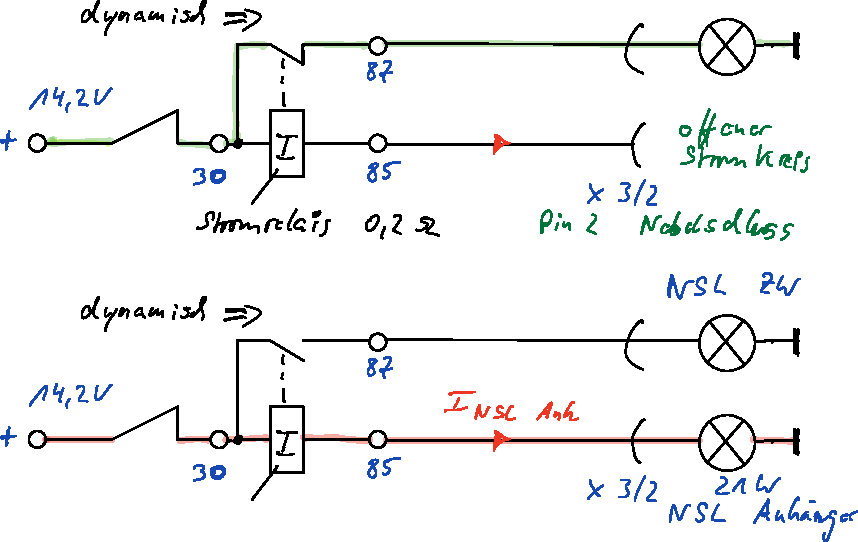
\includegraphics[width=0.6\textwidth]{images/Skizze/10_Stromrelais_Skizze.pdf}
\caption{Stromrelais}
%\label{fig:}%% anpassen
\end{figure}

\textbf{Rechenbeispiel}

geg:

$R_{Sp} = 0,2~\Omega, R_{La} = 6,85~\Omega$

$U_{ges} = 14,2~V$

ges: $R_{ges}, I, U_{K_{Sp}}, U_{K_{La}}, P$

Formel

$R_{ges} = R_{Sp} + R_{La}$

$I = \frac{U_{ges}}{R_{ges}}$

$U_{K_{Sp}} = R_{Sp} \cdot I, U_{K_{La}} = R_{La} \cdot I$

$P = U_{K_{La}} \cdot I$

Lösung:

$R_{ges} = 7,05~\Omega$

$I = 2,0142~A$

$U_{K_{Sp}} = 0,4028~V, U_{K_{La}} = 13,7972~V$

$P = 7,79~W$

\subsection{Reedkontaktschalter,
Reedrelais}\label{reedkontaktschalter-reedrelais}

Schaltzeichen Fachbuch (\textcite{brand:2020:fachkundeKfz} S. 681)

\begin{figure}[!ht]% hier: !ht
\centering
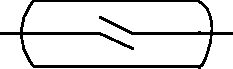
\includegraphics[width=0.1\textwidth]{images/Skizze/12_Reedkontaktschalter_Skizze.pdf}
\caption{Reedkontaktschalter}
%\label{fig:}%% anpassen
\end{figure}

\textbf{Einsatzmöglichkeiten}

\begin{enumerate}
\item
  Füllstandsanzeige

  \begin{itemize}
  \item
    Wischwasser
  \item
    Kühlwasser
  \end{itemize}
\item
  Glühkerzenausfallkontrolle
\item
  Geschwindigkeitssensor
\end{enumerate}

\subsection{Schrittrelais, Stromstoßrelais
(Stromsparen)}\label{schrittrelais-stromstossrelais-stromsparen}

\begin{figure}[!ht]% hier: !ht
\centering
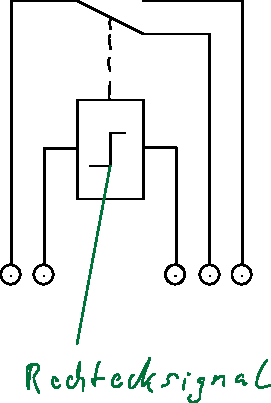
\includegraphics[width=0.15\textwidth]{images/Skizze/11_Schrittrelais_Skizze.pdf}
\caption{Schrittrelais}
%\label{fig:}%% anpassen
\end{figure}

keine Prüfung

bistabiles Relais (BMW)

\newpage

\section{Spannungsverlust - Spannungsfall - Spannungsabfall
(Prüfung)}\label{spannungsverlust-spannungsfall-spannungsabfall-pruefung}

$U_v = u$

Nennquerschnitt Tabellenbuch (\textcite{bell:2021:tabellenbuchKfz} S. 280)

Klemmbezeichnung Tabellenbuch (\textcite{bell:2021:tabellenbuchKfz} S. 273)

Spannungsfall Tabellenbuch (\textcite{bell:2021:tabellenbuchKfz} S. 280)

\begin{figure}[!ht]% hier: !ht
\centering
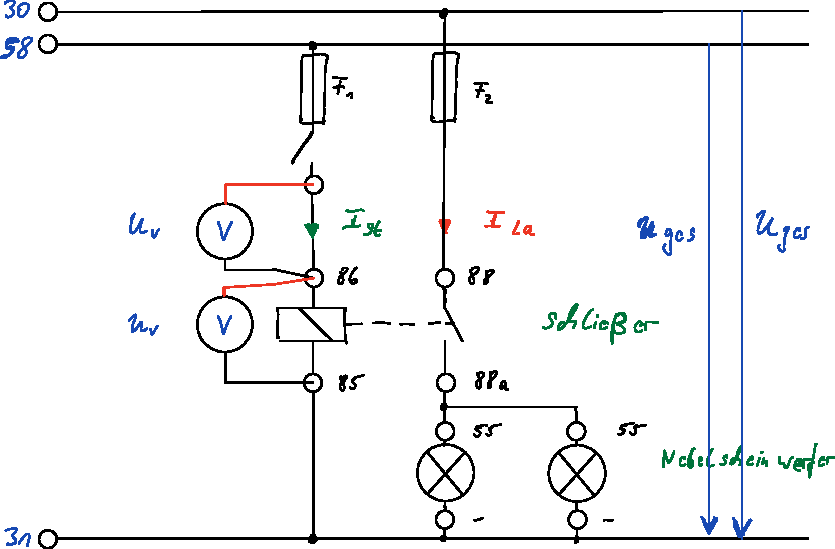
\includegraphics[width=0.65\textwidth]{images/Skizze/13_Spannungsverlust_Skizze.pdf}
\caption{Spannungsverlust}
%\label{fig:}%% anpassen
\end{figure}

\begin{table}[!ht]% hier: !ht 
\centering 
	\caption{}% \label{tab:}%% anpassen 
\begin{tabular}{@{}lll@{}}
\hline
\textbf{Bezeichnung} & \textbf{Benennung} & \textbf{Einheit} \\
\hline
$U_{ges}$ & Gesamtspannung & $[V]$ \\
$U_v$ & Spannungsverlust & $[V]$ \\
$U_k$ & Klemmspannung & $[V]$ \\
$R_l$ & Leiterwiderstand & $[\Omega]$ \\
$I$ & Stromfluss, Stromstärke & $[A]$ \\
\hline
\end{tabular} 
\end{table}

$U_{ges} = U_v + U_k;\, U_k = U_{ges} - U_v;\, U_v = U_{ges} - U_k$

$U_v = R_l \cdot I; R_l = \frac{\rho \cdot l}{A} \quad \bigl[\frac{\Omega \cdot mm^2 \cdot m}{m \cdot mm^2}\bigl] = \Omega$

$U_k = U_{ges} - R_l \cdot I$

$\boxed{U_v = \frac{\rho \cdot l \cdot I}{A}} \quad \bigl[\frac{\Omega \cdot mm^2 \cdot m \cdot A}{m \cdot mm^2}\bigl] = V$

$U_{v_{~\%}} = \frac{U_v \cdot 100}{U_{ges}} \quad \bigl[\frac{V \cdot ~\%}{V}\bigl] = ~\%$

$\boxed{U_{v_{max}} = 0,5~V}$

$\boxed{\text{max. Leiterwiderstand} = 1~\Omega}$ (außer
Starterhauptleitung)

\textbf{Spannungsfall} $U_v$ in einem stromdurchflossenen Leiter
entsteht infolge des Leiterwiderstandes ein Spannungsfall, der sich am
Verbraucher als Verlust auswirkt.

\textbf{Leiterquerschnitt} $A$ der Mindestquerschnitt einer Leitung
richtet sich nach der Stromstärke, der Leiterlänge, dem spezifischen
Widerstand des Leitermaterials und dem zulässigen Spannungsfall. Wegen
der Erwärmung des Leiters muss gegebenenfalls die Stromdichte
nachgeprüft werden.

\newpage

\section{Innenwiderstand von
Spannungsquellen}\label{innenwiderstand-von-spannungsquellen}

\begin{figure}[!ht]% hier: !ht
\centering
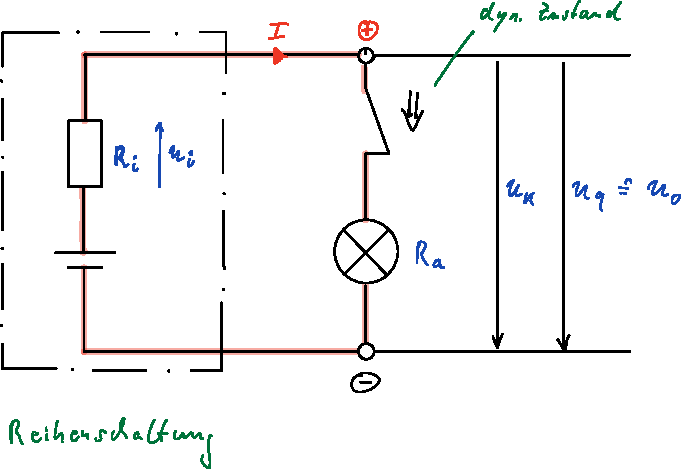
\includegraphics[width=0.6\textwidth]{images/Skizze/14_ Innenwiderstand_von_Spannungsquellen_Skizze.pdf}
\caption{Innenwiderstand von Spannungsquellen}
%\label{fig:}%% anpassen
\end{figure}

\begin{table}[!ht]% hier: !ht 
\centering 
	\caption{}% \label{tab:}%% anpassen 
\begin{tabular}{@{}lll@{}}
\hline
\textbf{Bezeichnung} & \textbf{Benennung} & \textbf{Einheit} \\
\hline
$U_q$ & Quellspannung & $[V]$ \\
$U_0 (U_{Null})$ & Leerlaufspannung & $[V]$ \\
$U_k$ & Klemmenspannung (Last, mit Verbraucher) & $[V]$ \\
$U_i$ & Spannungsabfall am Innenwiderstand & $[V]$ \\
$R_i$ & Innenwiderstand & $[\Omega]$ \\
$R_a$ & Außenwiderstand & $[\Omega]$ \\
$I$ & Stromfluss, -stärke & $[A]$ \\
\hline
\end{tabular} 
\end{table}

\textbf{Innenwiderstand} $R_i$ ist die Summe der Innenwiderstände der
Zellen. Er ist u. a. von der Temperatur und dem Lade- beziehungsweise
Entladezustand abhängig. Die Klemmenspannung $U_k$ der belasteten
Batterie ist deshalb um den Spannungsfall niedriger als die
Leerlaufspannung $U_0$.

$U_q = U_k + U_i \quad [V + V] = V$

$U_k = U_q - U_i \quad [V - V] = V$

$U_i = U_q - U_k \quad [V - V] = V$

$U_i = I \cdot R_i \quad [A \cdot \Omega] = V$

$U_k = I \cdot R_a \quad [A \cdot \Omega] = V$

$I = \frac{U_i}{R_i} \quad [\frac{V}{\Omega}] = A$

$I = \frac{U_k}{R_a} \quad [\frac{V}{\Omega}] = A$

$I = \frac{U_q}{R_{ges}} \quad [\frac{V}{\Omega}] = A$

$I = \frac{U_q}{R_i + R_a} \quad [\frac{V}{\Omega + \Omega}] = A$

$\boxed{U_k = U_q - I \cdot R_i} \quad [V - A \cdot \Omega \rightarrow V - V] = V$

$\boxed{R_i = \frac{U_i}{I}} \quad [\frac{V}{A}] = \Omega$

\textbf{Rechenbeispiel}

geg:

$U_q = 12~V, U_k = 9,6~V$

$R_a = 2,618~\Omega$ (Außenwiderstand)

ges: $I, R_i$

Formel:

$I = \frac{U_k}{R_a}$

$R_i = \frac{U_{R_i}}{I} \to R_i = \frac{(U_q - U_k)}{I}$

Lösung:

$I = 3,6669~A$

$R_i = 0,6545~\Omega$

\newpage

\section{Parallelschaltung von
Widerständen}\label{parallelschaltung-von-widerstaenden}

\begin{figure}[!ht]% hier: !ht
\centering
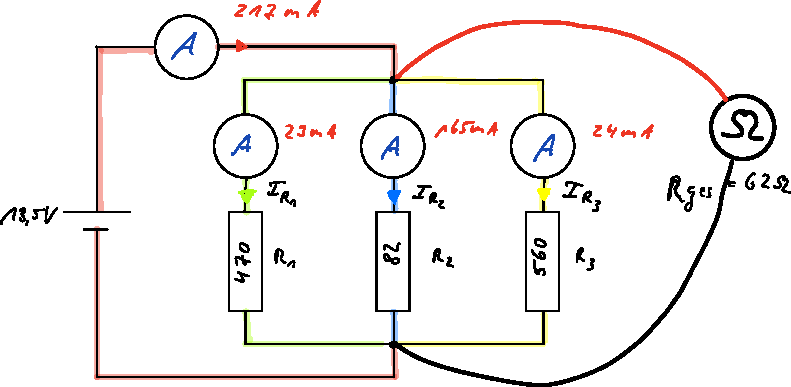
\includegraphics[width=0.6\textwidth]{images/Skizze/19_Parallelschaltung_Widerstaende_Skizze.pdf}
\caption{Parallelschaltung von Widerstände}
%\label{fig:}%% anpassen
\end{figure}

Werden mehrere verschiedene - oder gleich große Widerstände parallel
geschaltet, so fließt durch jeden Widerstand, nach Größe des
Widerstandes ein Strom, der addiert den Gesamtstrom ergibt.

$I_{ges} = I_{R_1} + I_{R_2} + I_{R_3} + \dots + I_{R_n} \quad [A + A + A] = A$

An jeden parallel geschalteten Widerstand liegt die gleiche Spannung an.

$U_{ges} = U_{R_1} = U_{R_2} = U_{R_3} = \dots = U_{R_n} \quad [V = V = V] = V$

Der Gesamtwiderstand ist stets kleiner als der kleinste
Einzelwiderstand.

$R_{ges} = \frac{1}{\frac{1}{R_1} + \frac{1}{R_2} + \frac{1}{R_3} + \dots + \frac{1}{R_n}} \quad \bigl[\frac{1}{\frac{1}{\Omega} + \frac{1}{\Omega} + \frac{1}{\Omega}} = \frac{1}{\frac{1}{\Omega}} = \frac{1}{S}\bigl] = \Omega$

Möchte Mann/Frau den Gesamtwiderstand von gleich großen parallel
geschalteten Widerständen berechnen, kann nachfolgende Gleichung
angewendet werden.

$R_{ges} = \frac{R_{Teil}}{n} \quad \bigl[\frac{\Omega}{1}\bigl] = \Omega \quad \to n = \frac{R_{Teil}}{R_{ges}} \quad \bigl[\frac{\Omega}{\Omega}\bigl] = 1$

n = Anzahl der Widerstände (gleich große Widerstände)

$R_{ges} = \frac{R_1 \cdot R_2}{R_1 + R_2}$

$R_{ges} = \frac{1}{\frac{1}{R_1} + \frac{1}{R_2} + \frac{1}{R_3}}$

$\to R_{1} = \frac{1}{\frac{1}{R_{ges}} - \frac{1}{R_2} - \frac{1}{R_3}} \quad \to R_{2} = \frac{1}{\frac{1}{R_{ges}} - \frac{1}{R_1} - \frac{1}{R_3}} \quad \to R_{3} = \frac{1}{\frac{1}{R_{ges}} - \frac{1}{R_1} - \frac{1}{R_2}}$

\textbf{Rechenbeispiel}

geg: \textbar\textbar{}

$U = 13,5~V$ (Hinweis: $U_{ges} = U$)

$R_1 = 470~\Omega, R_2 = 82~\Omega, R_3 = 560~\Omega$

ges: $I_{ges}, I_1, I_2, I_3, R_{ges}$

Formel:

$I_1 = \frac{U}{R_1}, I_2 = \frac{U}{R_2}, I_3 = \frac{U}{R_3}$

$I_{ges} = I_1 + I_2 + I_3$

$R_{ges} = \frac{U}{I_{ges}}$

Lösung:

$I_1 = 0,0287~A, I_2 = 0,1646~A, I_3 = 0,0241~A$

$I_{ges} = 0,2175~A$

$R_{ges} = 62,079~\Omega$

\newpage

\section{gemischte Schaltung}\label{gemischte-schaltung}

\begin{figure}[!ht]% hier: !ht
\centering
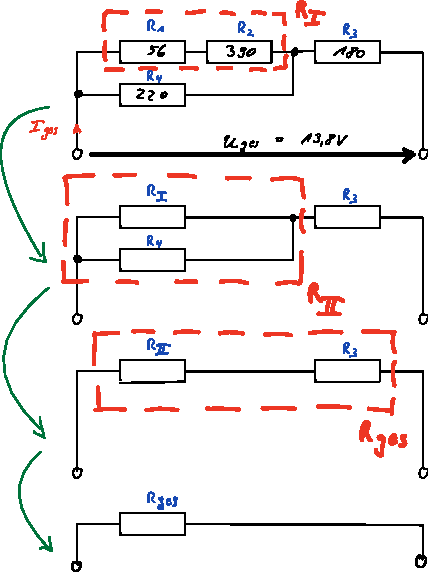
\includegraphics[width=0.6\textwidth]{images/Skizze/25_gemischte_Schaltung.pdf}
\caption{gemischte Schaltung}
%\label{fig:}%% anpassen
\end{figure}

$R_\mathrm{I} = R_1 + R_2$

$R_\mathrm{II} = \frac{1}{\frac{1}{R_\mathrm{I}} + \frac{1}{R_4}}$

$R_{ges} = R_\mathrm{II} + R_3$

Gemischte Schaltungen berechnet man, indem man sie in Reihen- und
Parallelschaltungen zerlegt und Ersatzwiderstände bildet.

\textbf{Rechenbeispiel}

geg:

$R_1 = 56~\Omega, R_2 = 390~\Omega, R_3 = 180~\Omega, R_4 = 220~\Omega$

$U_{ges} = 13,8~V$

ges: $U_{Teil}, R_{Teil}, I_{Teil}, I_{{ges}}, R_{ges}$

Formel:

$R_I = R_1 + R_2$

$R_{II} = \frac{1}{\frac{1}{R_I} + \frac{1}{R_4}}$

$R_{ges} = R_{II} + R_3$

$I_{ges} = \frac{U_{ges}}{R_{ges}}$

$U_{R_3} = R_3 \cdot I_{ges}$

$U_{R_{II}} = R_{II} \cdot I_{ges}$

$I_{R_I} = \frac{U_{R_{II}}}{R_I}$

$I_{R_4} = \frac{U_{R_{II}}}{R_4}$

$U_{R_1} = R_1 \cdot I_{R_I}$

$U_{R_2} = R_2 \cdot I_{R_I}$

Lösung:

$R_I = 446~\Omega, R_{II} = 147,3273~\Omega$

$R_{ges} = 327,3273~\Omega$

$I_{ges} = 0,0422~A$

$U_{R_3} = 7,5887~V, U_{R_{II}} = 6,2113~V$

$I_{R_I} = 0,0139~A, I_{R_4} = 0,0282~A$

$U_{R_1} = 0,7799~V, U_{R_2} = 5,4314~V$

\newpage

\section{Die elektrische Leistung}\label{die-elektrische-leistung}

$P$ (Power) Watt, $[W], [kW]$

\emph{schottischer Ingenieur James Watt (1736-1819)}

Glühlampe $12~V/21~W$, Wärmestrahlerbeleuchtungskörper

\begin{figure}[!ht]% hier: !ht
\centering
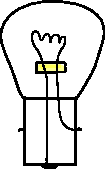
\includegraphics[width=0.12\textwidth]{images/Skizze/26_Leistung_Gluehlampe.pdf}
\caption{Leistung Glühlampe}
%\label{fig:}%% anpassen
\end{figure}

$\boxed{P = U \cdot I} \quad [V \cdot A] = W$

$\boxed{U = \frac{P}{I}} \quad [\frac{W}{A} \to \frac{V \cdot A}{A}] = V$

$\boxed{I = \frac{P}{U}} \quad [\frac{W}{V} \to \frac{V \cdot A}{V}] = A$

\textbf{wenn $I$ fehlt} (Einsetzverfahren)

$P = U \cdot I \quad [V \cdot A] = W, \quad I = \frac{U}{R} \quad [\frac{V}{\Omega}] = A$

$P = U \cdot \frac{U}{R} \to \boxed{P = \frac{U^2}{R}} \quad [\frac{V \cdot V}{\Omega} \to A \cdot V] = W$

\textbf{wenn $U$ fehlt} (Einsetzverfahren)

$P = U \cdot I \quad [V \cdot A] = W, \quad U = R \cdot I \quad [\Omega \cdot A] = V$

$P = R \cdot I \cdot I \to \boxed{P = R \cdot I^2} \quad [\Omega \cdot A \cdot A \to V \cdot A] = W$

Die elektrische Leistung $P$ ist das Produkt aus Spannung $U$ und
Strom $I$.

\textbf{Anmerkung} die verschiedenen Leistungen der unterschiedlichen
Verbraucher, in Schaltungen, addieren sich zur Gesamtleistung.

\textbf{Merke} halbe Spannung bedeutet nicht halbe Leistung und
umgekehrt halbe Leistung bedeutet nicht halbe Spannung, die Leistung
ändert sich im Quadrat.

Bei der Berechnung an/von Wärmestrahlerbeleuchtungskörpern, zuerst den
Widerstand berechnen.


	%%%%%%%%%%%%%%%%%%%%%%%%%%%%%%%%%%%%%%%%%%%%%%%%%%%%%%%%%%%%%%%%%%
    % Bibliographie
    \printbibliography
\end{document}
